
\begin{center}
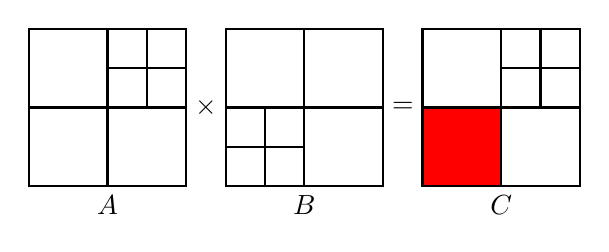
\begin{tikzpicture}[scale=0.5]
  %% matrix A
  \draw[ thick] (0,0) rectangle (4.0,4.0);
  \draw[ thick] (0,0) rectangle (2.0,2.0);
  \draw[ thick] (2.0,2.0) rectangle (4.0,4.0);
    \draw[ thick] (2.0,2.0) rectangle (3.0,3.0);
    \draw[ thick] (3.0,3.0) rectangle (4.0,4.0);
    \draw[ thick] (2.0,4.0) rectangle (3.0,3.0);
    \draw[ thick] (3.0,3.0) rectangle (4.0,2.0);
  \draw[ thick] (0,4.0) rectangle (2.0,2.0);
  \draw[ thick] (2.0,2.0) rectangle (4.0,0.0);

  %% matrix B
  \draw[ thick] (5.0,0) rectangle (9.0,4.0);
  \draw[ thick] (5.0,0) rectangle (7.0,2.0);
    \draw[ thick] (5.0,0) rectangle (6.0,1.0);
    \draw[ thick] (6.0,1.0) rectangle (7.0,2.0);
    \draw[ thick] (7.0,0) rectangle (6.0,1.0);
    \draw[ thick] (6.0,1.0) rectangle (5.0,0.0);
  \draw[ thick] (7.0,2.0) rectangle (9.0,4.0);
  \draw[ thick] (5,4.0) rectangle (7.0,2.0);
  \draw[ thick] (7.0,2.0) rectangle (9.0,0.0);

  %% matrix C
  \filldraw[ fill=red, draw=black] (10.0,0.0) rectangle (12.0,2.0);
  \draw[thick] (10.0,0) rectangle (14.0,4.0);
  \draw[thick] (10.0,0) rectangle (12.0,2.0);
  \draw[thick] (12.0,2.0) rectangle (14.0,4.0);
    \draw[thick] (12.0,2.0) rectangle (13.0,3.0);
    \draw[thick] (13.0,3.0) rectangle (14.0,4.0);
    \draw[thick] (12.0,4.0) rectangle (13.0,3.0);
    \draw[thick] (13.0,3.0) rectangle (14.0,2.0);
  \draw[thick] (10.0,4.0) rectangle (12.0,2.0);
  \draw[thick] (12.0,2.0) rectangle (14.0,0.0);

  %% A
  \node at (4.5,2.0) {$\times$};
  \node at (9.5,2.0) {$=$};
  \node[below] at (12.0,0.0) {$C$};
  \node[below] at (7.0,0.0) {$B$};
  \node[below] at (2.0,0.0) {$A$};

\end{tikzpicture}
\end{center}

